\documentclass[a4paper]{article}
\usepackage[pdftex]{graphicx}
\usepackage[utf8]{inputenc}
\usepackage{enumerate}
\usepackage{amssymb}
\usepackage{eurosym}
\usepackage{icomma}
\usepackage{siunitx}
\sisetup{locale=DE} 
\usepackage{tikz}
\usepackage{href-ul}
\hypersetup{
	colorlinks=true,
	linkcolor=blue,
	urlcolor=blue}
\usepackage{geometry}
\geometry{a4paper, top=15mm, left=15mm, right=15mm, bottom=15mm,
	headsep=10mm, footskip=12mm}

\begin{document}
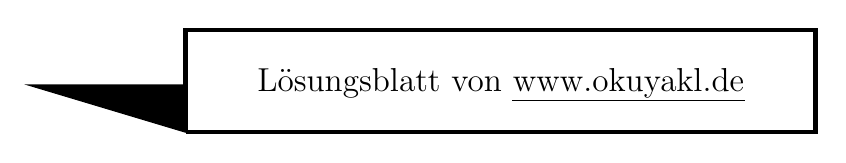
\begin{tikzpicture}(10,3)
	\draw[ultra thick](2,0) --(10,0) -- (10,1.3) --(2,1.3) -- (2,0);
	\draw[fill=black](2,0)-- (0,.6) -- (2,.6) -- (2,0);
	\node at (6,.6) {\large Lösungsblatt von \href{https://www.okuyakl.de}{www.okuyakl.de}};
\end{tikzpicture}
\vspace{0.5 cm}


\renewcommand{\arraystretch}{2.5}
\begin{tabular}{|c|p{13 cm}|}
\hline
$>\SI{1000}{\tonne}$ & Containerschiff \\	
\hline	
$\SI{100}{\tonne}$ bis $\SI{1000}{\tonne}$ & Lok, Airbus A380\\
\hline
$\SI{10}{\tonne}$ bis $\SI{100}{\tonne}$ & Brontosaurus, LKW \\
\hline	
$\SI{1}{\tonne}$ bis $\SI{10}{\tonne}$ & Auto, Traktor \\
\hline
$\SI{100}{\kilogram}$ bis $\SI{1}{\tonne}$ & Pferd, Motorrad  \\
\hline
$\SI{10}{\kilogram}$ bis $\SI{100}{\kilogram}$ & Getränkekiste, Fahrrad\\
\hline
$\SI{1}{\kilogram}$ bis $\SI{10}{\kilogram}$ & Laptop, Schultasche  \\
\hline
$\SI{100}{\gram}$ bis $\SI{1}{\kilogram}$ & Fußball, Taube\\
\hline
$\SI{10}{\gram}$ bis $\SI{100}{\gram}$ & Schokoriegel, Batterie AA \\
\hline
$\SI{1}{\gram}$ bis $\SI{10}{\gram}$ & 1-Cent-Münze, Spielwürfel, Bleistift\\
\hline
$\SI{100}{\milli\gram}$ bis $\SI{1}{\gram}$ & Spickzettel, Bohne \\
\hline
$\SI{10}{\milli\gram}$ bis $\SI{100}{\milli\gram}$ & Grashalm, Briefmarke \\
\hline
$\SI{1}{\milli\gram}$ bis $\SI{10}{\milli\gram}$ & Tannennadel, Reiskorn\\
\hline
$< \SI{1}{\milli\gram}$ &  Haar, Sandkorn \\
\hline
\end{tabular}


\begin{center}
	\includegraphics[width=7 cm]{../../viecher/endcomic.pdf}
	
	Hier geht es zurück zum \href{https://www.okuyakl.de/phys/p7ggrL005/aa005.pdf}{Aufgabenblatt}
\end{center}


\end{document}

